\documentclass[12pt]{article}

\usepackage[spanish]{babel}

\usepackage{amsmath}
\usepackage{amssymb}

\usepackage{hyperref}
\usepackage{graphicx}
\usepackage{listings}
\usepackage{color}
\usepackage{multicol}
\usepackage{enumitem}
\usepackage{here}
\usepackage{dsfont}
\usepackage{tipa}
\usepackage{float}
\usepackage{dsfont} 
\spanishdecimal{.}

\title{Matemáticas para las Ciencias Aplicadas II}
\title{
        \textbf{Tarea 03} \\
        \vspace{1ex}
        \large Matemáticas para las Ciencias Aplicadas II \\
        Facultad de Ciencias, UNAM}
\date{\today}
\author{Flores Morán Julieta Melina \\ Zarco Romero José Antonio}

\begin{document}
\maketitle

% 1 -------------------------------------------------------------------------------------------------------------
\section{}

Sea la función escalar de variable vectorial $$f(x,y,z)= \sqrt{x} +\sqrt{y} +\sqrt{z} + \ln{(4-x^2-y^2-z^2)}$$.

\begin{itemize}[format=\textbf]

\item Evalúe $f(1,1,1)$.

\begin{align*}
f(1,1,1)
&= \sqrt{1} +\sqrt{1} +\sqrt{1} + \ln{(4-1^2-1^2-1^2)} \\
&= 1+1+1+ \ln{(4-1-1-1)} \\
&= 1+1+1+ \ln{1} \\
&= 1+1+1+0 \\
&= 3
\end{align*}

\item Determine y describa el dominio de $f(x, y, z)$.

\begin{align*}
D
&=\{(x,y,z)~|~x \geq 0, y \geq 0, z \geq 0, (4-x^2-y^2-z^2) > 0\} \\
\therefore D
&= \{(x,y,z)~|~x \geq 0, y \geq 0, z \geq 0, (x^2+y^2+z^2) < 4\}
\end{align*}

La desigualdad $x^2+y^2+z^2<4$, describe los puntos $(x,y,z)$ que quedan dentro de la región definida por la esfera de radio $r=2$ centrada en el origen.

\end{itemize}

% 2 -------------------------------------------------------------------------------------------------------------
\section{}

Se muestran las curvas de nivel \textbf{isotermas} para la temperatura del agua $[C]$ en un lago en el año 1998 como una función de la profundidad y el tiempo en años. Estime la temperatura en el lago el 9 de junio (día 160) a una profundidad de 10 \textit{metros} y el día 29 de junio (día 180) a una profundidad de 5 \textit{metros}.

\begin{figure}[H]
  \centering
  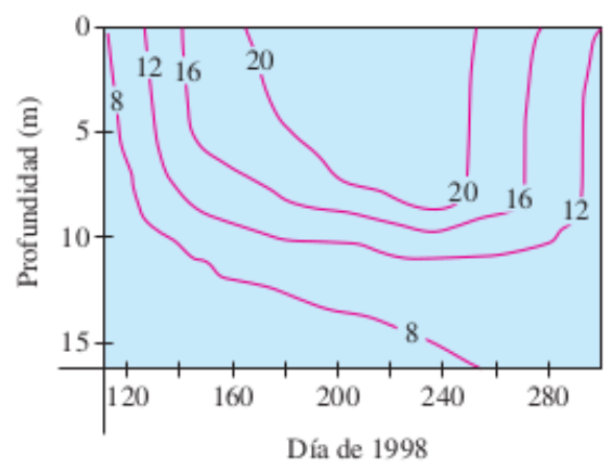
\includegraphics[width=0.7\textwidth]{./img/t3_ej2.png}
\end{figure}

Sea $f(x, y)$ la función para la temperatura del agua $[C]$, donde $x$ es el día de 1988 y $y$ es la profundidad en $(m)$, tenemos que: \\

El punto $(160,10)$ queda entre las curvas de nivel con valores de temperatura del agua $[C]$ de 8 y 12. Dado que el punto parece estar ubicado $\frac{3}{4}$ de distancia de 8 a 12, estimamos que $$f(160,10) \approx 11$$

$\therefore {11}^\circ C$ es la estimación de la temperatura en el lago el 9 de junio (día 160) a una profundidad de 10 \textit{metros}.

El punto $(180,5)$ queda entre las curvas de nivel con valores de temperatura del agua $[C]$ de 16 y 20. Dado que el punto se encuentra muy próximo a 20, estimamos que $$f(180,5) \approx 19.5$$

$\therefore {19.5}^\circ C$ es la estimación de la temperatura en el lago el día 29 de junio (día 180) a una profundidad de 5 \textit{metros}.

% 3 -------------------------------------------------------------------------------------------------------------
\section{}

Determine los siguientes \textbf{límites}, si existen, o demuestren que no existen:

\begin{itemize}[format=\textbf]

  % 14.2, 7
\item $$\lim_{(x,y) \to (0,0)} \frac{4-xy}{x^2+3y^2}$$

  % 14.2, 9
\item $$\lim_{(x,y) \to (0,0)} \frac{x^4-4y^2}{x^2+2y^2}$$

  Sea $f(x,y) = \frac{x^4-4y^2}{x^2+2y^2}$. Primero nos aproximamos a $(0,0)$ por el eje $x$. Entonces $y=0$ da $f(x,0)=\frac{x^4}{x^2}=x^2$ para toda $x \neq 0$ de modo que 
  \begin{align*}
    f(x,y) \rightarrow 0 ~~ \text{ cuando }~~ (x,y) \rightarrow (0,0) ~~ \text{por el eje }x
  \end{align*}
  Ahora nos aproximamos por el eje $y$ haciendo $x=0$. Entonces $f(0,y) =  \frac{-4y^2}{2y^2}=-2$ para toda $y \neq 0$, de modo que
  \begin{align*}
    f(x,y) \rightarrow -2 ~~ \text{ cuando }~~ (x,y) \rightarrow (0,0) ~~ \text{por el eje }y
  \end{align*}

  $\therefore$ Puesto que $f$ tiene dos límites diferentes a lo largo de dos rectas distintas, el límite dado no existe.

  % 14.2, 21
\item $$\lim_{(x,y,z) \to (0,0,0)} \frac{xy+yz^2+xz^2}{x^2+y^2+z^4}$$

  Sea $f(x,y,z) =  \frac{xy+yz^2+xz^2}{x^2+y^2+z^4}$. Primero nos aproximamos a $(0,0,0)$ por el eje $x$. Entonces $y=z=0$ da $f(x,0,0)= \frac{0}{x^2}$ para toda $x \neq 0$ de modo que 
  \begin{align*}
    f(x,y,z) \rightarrow 0 ~~ \text{ cuando }~~ (x,y,z) \rightarrow (0,0,0) ~~ \text{por el eje }x
  \end{align*}
  Ahora, aproximémonos a $(0, 0,0)$ a lo largo de otra recta, digamos, $y=x$. Entonces $z=0$ da $f(x,x,0)= \frac{x\cdot x}{x^2+x^2}= \frac{x^2}{2x^2}=\frac{1}{2}$ para toda $x\neq 0$ de modo que 
  \begin{align*}
    f(x,y,z) \rightarrow \frac{1}{2} ~~ \text{ cuando }~~ (x,y,z) \rightarrow (0,0,0) ~~ \text{por la recta }y=x
  \end{align*}

$\therefore$ Puesto que hemos obtenido distintos límites en distintas trayectorias,
el límite dado no existe.

\end{itemize}

% 4 -------------------------------------------------------------------------------------------------------------
\section{}

La temperatura \textbf{T} en [Celsius] en un lugar del hemisferio norte depende de la longitud $x$, latitud $y$, y el tiempo $t$ de modo que podemos escribir $T(x, y, t)$. Mida el tiempo en horas a partir del inicio de enero.

\begin{itemize}[format=\textbf]

\item Explique ¿qué significan las derivadas parciales $\frac{\partial T}{\partial x}, \frac{\partial T}{\partial y}$ y $\frac{\partial T}{\partial t}$?

\item Honolulu tiene una longitud de $158^{\circ}$ W y una latitud de $21^{\circ}$ N. Suponga que a las 9:00 AM el primero de enero, los vientos empujan aire caliente hacia el noreste, de modo que el aire del oeste y del sur es caliente y el aire del norte y el este es más frío. ¿Esperaria que $f_x(158, 21, 9)$, $f_y(158, 21, 9)$ y $f_t(158, 21, 9)$ sean positivas o
negativas? Explique.

\end{itemize}

% 5 -------------------------------------------------------------------------------------------------------------
\section{}

Use la definición de las \textbf{derivadas parciales} como límites para determinar $f_x(x, y), f_y(x, y)$ de la función:

\begin{itemize}[format=\textbf]

\item $$f(x, y) = xy^2 - x^3y$$

  Recordemos que, para determinar $f_x$, debemos conservar a $y$ constante y derivar $f (x, y)$ con respecto a $x$. Así, se obtiene que
  \begin{align*}
    f_x(x,y)
    &= \lim_{h\to 0} \frac{f(x+h,y)-f(x,y)}{h} \\
    &= \lim_{h\to 0} \frac{(x+h)y^2 - (x+h)^3y- (xy^2 - x^3y)}{h} \\
    &= \lim_{h\to 0} \frac{xy^2+y^2h - (x^3y+3x^2yh+3xyh^2+yh^3) - xy^2 + x^3y}{h} \\
    &= \lim_{h\to 0} \frac{xy^2+y^2h - x^3y - 3x^2yh -3xyh^2 -yh^3 - xy^2 + x^3y}{h} \\
    &= \lim_{h\to 0} \frac{hy^2 - 3x^2yh -3xyh^2y - yh^3}{h} \\
    &= \lim_{h\to 0} \frac{h(y^2 - 3x^2y -3xyh - yh^2)}{h} \\
    &= \lim_{h\to 0} (y^2 - 3x^2y - 3xyh - yh^2) \\
    &= y^2 - 3x^2y
  \end{align*}
    

  Asimismo, para determinar $f_y$, debemos conservar a $x$ constante y derivar $f(x,y)$ con respecto a $y$. De este modo, tenemos que
  \begin{align*}
    f_y(x,y)
    &= \lim_{h\to 0} \frac{f(x,y+h)-f(x,y)}{h} \\
    &= \lim_{h\to 0} \frac{x(y+h)^2 - x^3(y+h) - (xy^2 - x^3y)}{h} \\
    &= \lim_{h\to 0} \frac{xy^2 + 2xyh + xh^2 - x^3y - x^3h - xy^2 + x^3y}{h} \\
    &= \lim_{h\to 0} \frac{2xyh + xh^2 - x^3h}{h} \\
    &= \lim_{h\to 0} \frac{h(2xy + xh - x^3)}{h} \\
    &= \lim_{h\to 0} (2xy + xh - x^3) \\
    &= 2xy - x^3
  \end{align*}

\end{itemize}

% 6 -------------------------------------------------------------------------------------------------------------
\section{}

La ley de los gases para una mas fija $m$ de un \textit{gas ideal} a temperatura $T$, presión $P$ y volumen $V$ absoulutos es $P V = mRT$, donde $R$ es la constante de los gases. Demuestre que:
$$\frac{\partial P}{\partial V} \cdot \frac{\partial V}{\partial T} \cdot \frac{\partial T}{\partial P} = -1$$

% 7 -------------------------------------------------------------------------------------------------------------
\section{}

Determine una ecuación del \textbf{plano tangente} a la superficie dada en el punto solicitado:

\begin{itemize}[format=\textbf]

\item $z=3y^2-2x^2+x$, en el punto $(2,-1,-3)$.

Sea $f(x,y)=3y^2-2x^2+x$. Entonces 

\begin{align*}
f_x(x,y)=-4x+1 
&&
f_y(x,y)=6y \\
f_x(2,-1)=-7
&&
f_y(2,-1)=-6
\end{align*}

Entonces da la ecuación del plano tangente en $(2,-1,-3)$ como

\begin{align*}
z-(-3)&=(-7)(x-2)+(-6)(y-(-1)) \\
z+3&=-7(x-2)-6(y+1) \\
\text{o bien,}\\
z=-7x-6y+5
\end{align*}

\item $z=\sqrt{xy}$, en el punto $(1,1,1)$.

\end{itemize}

% 8 -------------------------------------------------------------------------------------------------------------
\section{}

Calcule la \textbf{aproximación lineal} de la función $f(x,y,z)=\sqrt{x^2+y^2+z^2}$ en el punto $(3,2,6)$ y con ella \textit{aproxime} el número $\sqrt{(3.02)^2+(1.97)^2+(5.99)^2}$.

% 9 -------------------------------------------------------------------------------------------------------------
\section{}

Utilice \textbf{diferenciales} para estimar la cantidad de \textit{estaño} en una lata cerrada de estaño cuyo diámetro es 8 \textit{cm} y altura 12 \textit{cm} si el estaño tiene
0.04 \textit{cm} de espesor.

% 10 -------------------------------------------------------------------------------------------------------------
\section{}

Mediante la \textbf{regla de la cadena} encuentre, dado que:

\begin{itemize}[format=\textbf]

\item $z=x^2y^3$, donde , $x=s \cos{t}$, $y=s \sin{t}$

\end{itemize}

% 11 -------------------------------------------------------------------------------------------------------------
\section{}

La temperatura en un punto $(x, y)$ es $T(x, y)$, medida en grados centigrados. Un insecto se arrastra de tal modo que su posición después de $t$ \textit{segundos} está dada por $x =
\sqrt{1 + t}$, $y = 2 + \frac{t}{3}$, donde $x$ e $y$ se miden en centimetros. La función temperatura satisface $T_x(2, 3) = 4$, $T_y(2, 3) = 3$.
¿Qué tan rapido se eleva la temperatura del insecto en su trayectoria después de 3 \textit{segundos}?

% 12 -------------------------------------------------------------------------------------------------------------
\section{}

Se muestran curvas de nivel para la \textit{presión barométrica} [mili-bares], para las 6 : 00 AM del 10 de noviembre de 1998. Una zona con una presión de
sólo $972 mb$ se mueve la región noreste de Iowa. La distancia a lo largo de la linea roja de K (Kearney, Nebraska) a S (Sioux City, Iowa) es 300 km. Estime el valor de la derivada direccional de la función presión en Kearney en la dirección de Sioux City. ¿Cuáles son las unidades de la \textbf{derivada
  direccional}?

\begin{figure}[H]
  \centering
  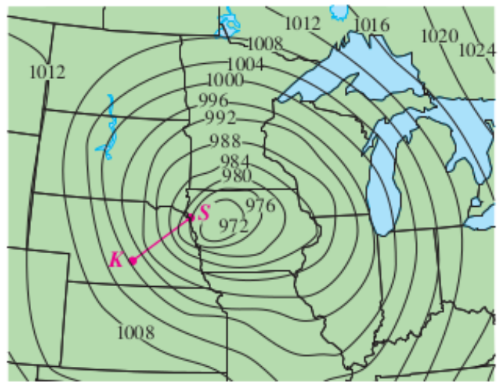
\includegraphics[width=0.7\textwidth]{./img/t3_ej12.png}
\end{figure}

% 13 -------------------------------------------------------------------------------------------------------------
\section{}

Sea $$f(x, y) = \sin{(2x + 3y)}, P(-6, 4), \vec{u}=\left(\frac{\sqrt{3}}{2},\frac{-1}{2} \right)$$

\begin{itemize}[format=\textbf]

\item Determine el gradiente de $f(x, y)$.

\item Evalue el \textbf{gradiente} en el punto $P$.

\item Encuentre la razón de cambio de $f(x, y)$ en $P$ en la dirección del vector $\vec{U}$.

\end{itemize}

\end{document}
